\documentclass[12pt,a4paper,]{scrreprt}
\usepackage[ngerman]{babel}
\usepackage[onehalfspacing]{setspace}
\usepackage[utf8]{inputenc}

\usepackage{graphicx,array,gnuplottex,siunitx,multicol,capt-of,amsmath,ulem,amsthm}
\let\phi\varphi
\setkomafont{chapter}{\fontsize{20bp}{22.2bp}\selectfont\bfseries}

\setkomafont{chapter}{\fontsize{14bp}{18.8bp}\selectfont\bfseries}
\setkomafont{section}{\fontsize{12bp}{14.4bp}\selectfont\bfseries}

\renewcommand{\chapterheadstartvskip}{\vspace*{-1\topskip}}
\renewcommand{\chapterheadendvskip}{\vspace*{0.8\topskip}}
%---------------------------------------------------------------------------------------------------------------------------------------------------------------
% Ende der Einstellungen
%---------------------------------------------------------------------------------------------------------------------------------------------------------------

%---------------------------------------------------------------------------------------------------------------------------------------------------------------
%Ab hier gibt es Inhalt
%---------------------------------------------------------------------------------------------------------------------------------------------------------------
\begin{document}

\title{Kugelfallviskosimeter}
\author{Henrik Jäger \\ 3114168 \and Lena Majer \\ 3115808}
\subtitle{S20a \\  Assistent: Patrik Zielinski}
\subject{Physikalisches Praktikum I}
\publishers{Universität Stuttgart}
\date{12. Januar 2017}
%\thanks{Assistent: Sascha Kolatschek}

\maketitle% Titelei

\tableofcontents   %Inhaltsverzeichnis
\pagebreak
\chapter{Einleitung}
\section{Ziel}
Bei diesem Versuch soll die Viskosität von Pumpenöl bestimmt werden. Nach Höppler wird die Viskosität mit Hilfe eines Kugelfallviskosmeters und bei variierter Temperatur bestimmt.
\section{Grundlagen}
Viskosität beschreibt die innere Reibung - die Zähigkeit – von Fluiden. Die Viskosität bei Gasen steigt mit zunehmender Temperatur. Bei Flüssigkeiten ist es genau anderst herum. Bei steigender Temperatur singt die Viskosität. Dies wird durch die Arrhenius- Andrade-Beziehung beschrieben: \\
\begin{equation}
\eta =c_1 \exp (c_2\cdot T{-1})
\end{equation}
$c_1$ und $c_2$ stellen Materialkonstanten dar. $c_2$ ist mit einer Aktivierungsenergie vergleichbar. Die absolute Temperatur T muss in Kelvin angegeben werden.\\
Sobald Gas schichten oder Flüssichkeitsschichten parallel zueinander bewegen, kommt es zu Reibungen, die großen Einfluss auf die Fortbewegung haben und zu Erniedrigung des Geschwindigkeitsgefälle führt.\\
Wird beispielweise eine Platte durch eine Flüssigkeit gezogen, muss die Flüssigkeit sich vor der Platte scheren. Hierbei kommt es zu zwischenmolekularen Kräften – den inneren Kräften. \\
Für eine laminare Strömung gilt nach Newton: \\
\begin{equation}
F_r = \eta \cdot A \cdot \frac{\partial v}{\partial x}
\end{equation}
Hierbei entspricht $\frac{\partial v}{\partial x}$ dem Geschwindichkeitsgefälle. A entspricht der eingetauchten Fläche.
Taucht der Begriff kinematische Viskosität auf,  versteht man damit die Definition:\\
\begin{equation}
V:=\frac{\eta}{\rho}
\end{equation}
$\rho$ entspricht der Dichte des verwendeten Fluids.\\
Als dynamische Viskosität wird mit $\eta$ bezeichnet. $\eta$ ist definiert als:\\
\begin{equation}
\eta  := \frac{\tau }{ \dot{\gamma} }
\end{equation}
Unter einer Laminaren Strömung versteht man eine Strömung ohne Verwirbelungen. Bei turbulenten Strömungen sind jedoch Verwirbelungen zu finden.\\
Markant zur Bestimmung, ob es sich um eine turbulente oder laminare Strömung handelt, ist die Reynoldszahl. Diese stellt ein Verhältnis zwischen Trägheitskräften und Zähigkeitkräften dar. Die Reynoldszahl ist definiert als:\\
Re = Beschleunigungsarbeit/ Reibungsarbeit \\
Bei Werten der Reynoldszahl $> Re_{krit}$ liegt eine Turbulente Strömung vor. Sind die Werte der Reynoldszahl $< Re_{krit}$  handelt es sich um eine laminare Strömung.\\
Bei laminarer Strömung kann das Gesetz von Hagen- Poiseulle verwendet werden. \\
\begin{equation}
I = \frac{\pi \cdot R^4}{8\cdot L\cdot\eta} \cdot \Delta p
\end{equation}
Um die Viskosität zu bestimmen gibt es zwei verschiedenen Vorgehensweisen nach Stokes oder nach Höppler. Nach Stokes wird die Auftriebskraft und die Stoksche Reibkraft sowie die Gewichtskraft betrachtet. Die Summe aller Kräfte muss nach Newton 0 ergeben.\\
Nach Höppler ist die Fallröhre kaum größer als die Kugel. Hierfür gilt:\\
\begin{equation}
\eta= K\cdot ( \varrho_k - \varrho_{Fl})\cdot t 
\end{equation}
K entspricht einer chiastischer Konstante für die Kugel.




\pagebreak

\chapter{Messprinzip mit Skizze und Versuchsablauf}
In diesem Versuch befindet sich Öl in einem Zylinder. Der Zylinder ist mit einer Kühler- flüssigkeit umgeben. Die Temperatur des Öles wird eingestellt. Nachdem die Temperatur 5 min konstant ist, wird eine Kugel durch das Öl fallen gelassen. Die Zeit, welche die Kugel für eine Strecke l benötigt wird gestoppt. Dies wird vier Mal wiederholt. Anschließend wird das Selbe bei vier weiteren Temperaturen wiederholt. Es wird von einer laminaren Strömung ausgegangen.
\begin{center}
	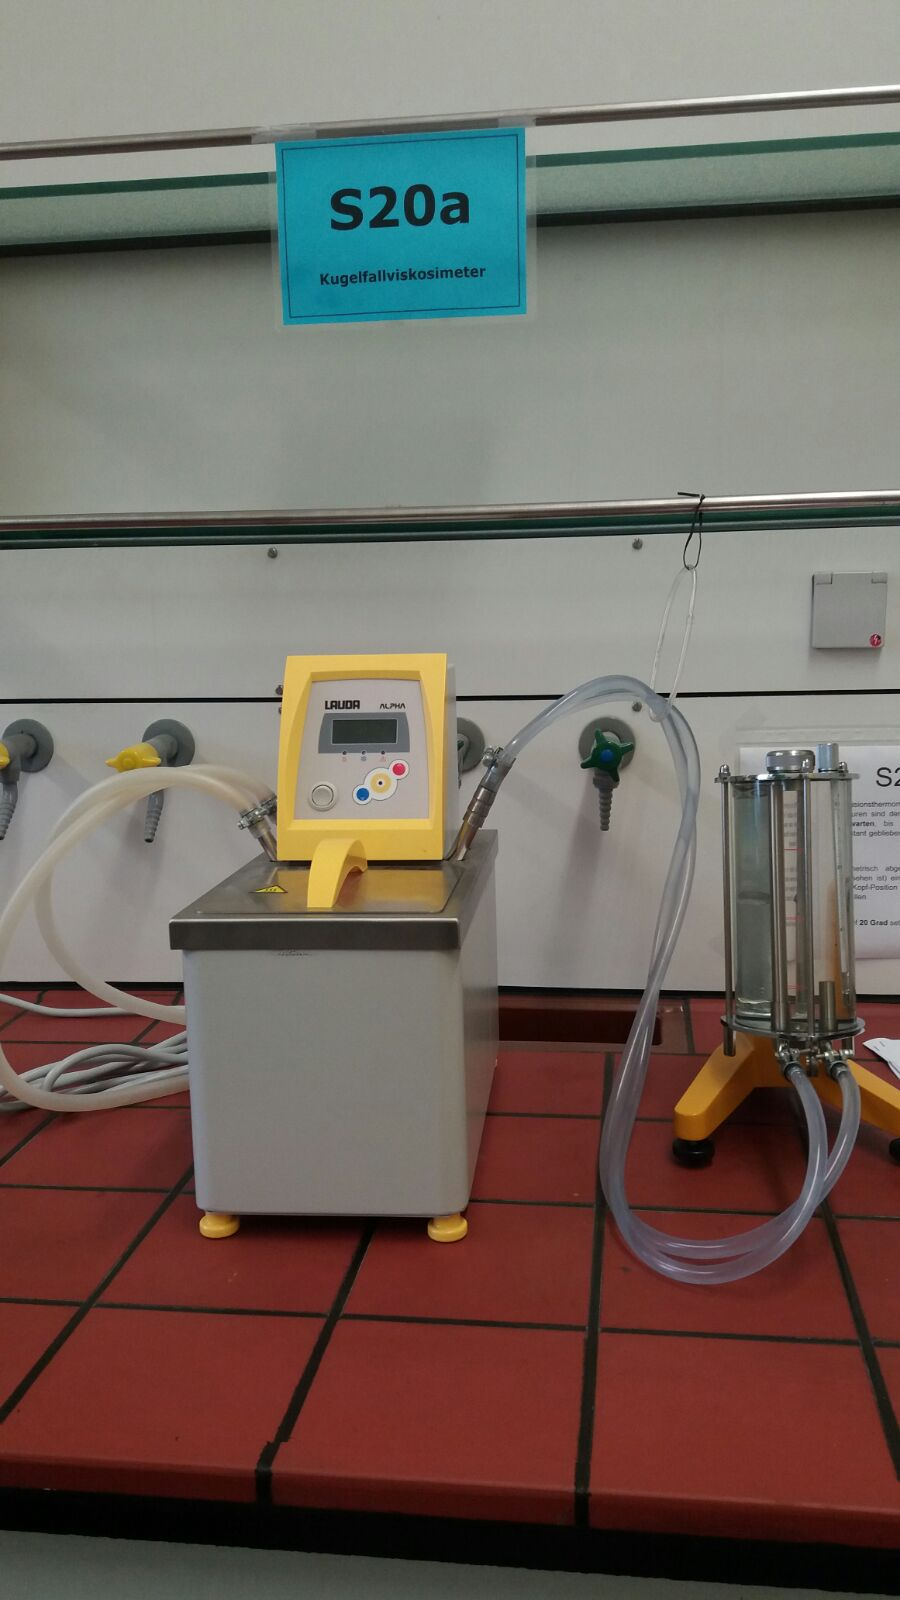
\includegraphics[scale=0.27]{aufbau.jpeg}
	\captionof{figure}[]{Versuchsaufbau}
\end{center}

	
\pagebreak

	\chapter{Formeln}
Nach Höppler ist die Fallröhre kaum größer als die Kugel. Hierfür gilt:\\
\begin{equation}
\eta= K\cdot(\rho_k - \rho_{Fl})\cdot t 
\end{equation}
K entspricht einer chiastischer Konstante für die Kugel.
Die Arrhenius-Andrade-Beziehung beziehung ist gegeben durch: \\
\begin{equation}
\eta =c_1 \exp (c_2 \cdot T^{-1})
\end{equation}
$c_1$ und $c_2$ stellen Materialkonstanten dar.
	

\pagebreak
	
	\chapter{Auswertung}
    	\section{Germanium- und Siliziumdioden in Durchlassrichtung}
        	\begin{gnuplot}[terminal=pdf,terminaloptions={font ",10" linewidth 2},scale=1.2]
            		set fit errorvariables
					
                  	set xlabel "Spannung [V]"
                  	set ylabel "Stromstärke [mA]"
					set xrange [0:1]
                    set yrange [0:1]
                    
                    f(x) = a*exp(b*x)
                    g(x) = c*exp(d*x)
                    fit f(x) "Daten/A1a.txt" using 2:1 via a,b
                    fit g(x) "Daten/A1a.txt" using 3:1 via c,d
                    
                  	plot "Daten/A1a.txt" using 2:1 title "Germanium", "Daten/A1a.txt" using 3:1 title "Silizium", f(x), g(x)
			\end{gnuplot}
        \captionof{figure}[DurchlassGerSil]{Kennlinien der Dioden in Durchlassrichtung}
        Im Diagramm wurde die Fitfunktion 			
        \begin{equation}
        	f(x) = a \cdot \exp(b\cdot x)
        \end{equation}
        verwendet. \\
        
        Wenn wir davon ausgehen, dass Formel \ref{Sperrstrom-vereinfacht} gilt, können wir den Sperrstrom aus den gefitteten Werten ermitteln. \\
        
        Es ergibt sich:
	\begin{center}
		\begin{tabular}{c|cc}
			&  Germanium & Silizium\\ \hline
    		$I_s$ & $0.3\cdot 10^{-3} mA$ &  $0.04\cdot 10^{-6} mA$
		\end{tabular}
    \end{center}    
   		     
        
        \pagebreak
        
        \section{Germanium- und Silizium in Sperrrichtung}
        \begin{gnuplot}[terminal=pdf,terminaloptions={font ",10" linewidth 2},scale=1.2]
        	set xlabel "Spannung [V]"
			set ylabel "Stromstärke [Mikroampere]"
            
			f(x)=a*x+b
            g(x)=c*x+d
            
            set key left
            
            set xrange [-8:0]
            
            fit f(x) "Daten/A1c.txt" using 1:2 via a,b
            fit g(x) "Daten/A1c.txt" using 1:3 via c,d
           	
            plot "Daten/A1c.txt" using 1:2 title "Germanium", "Daten/A1c.txt" using 1:3 title "Silizium", f(x), g(x)
                    
			\end{gnuplot}
        \captionof{figure}[DurchlassGerSil]{Kennlinien der Dioden in Sperrrichtung}
        
       \ \\
       Die Werte passen nicht zu den im ersten Versuchsteil bestimmten Sperrströmen
        \pagebreak
        
        \section{Zenerdiode in Durchlass- und Sperrrichtung}
        	Trägt man Durchlass und Sperrrichtungskennlinien in einem gemeinsamen Diagramm auf erhält man die Z-Linie. \\
        	\begin{gnuplot}[terminal=pdf,terminaloptions={font ",10" linewidth 2},scale=1.2]
					
                  	set xlabel "Spannung [V]"
                  	set ylabel "Stromstärke [Mikroampere]"
                  	
                  	plot "Daten/A2a.txt" using 2:1 title "Durchlassrichtung", "Daten/A2b.txt" using 1:2 title "Sperrrichtung 
			\end{gnuplot}
        \captionof{figure}[DurchlassGerSil]{Gesamtkennlinie der Zener-Diode} 
        \ \\
        Hier spielt in der Sperrrichtung die spezielle Eigenschaft der Zener-Diode eine Rolle. Ab einer gewissen Sperrspannung nimmt ihr differentieller Widerstand exponentiell zu, während er vor dieser Spannung noch nicht vorhanden war.\ \\
        Bei einer Spannung von $ U = 5,75 V$ wurde mit der $\mu A$ -Skala ein Strom von $948 \mu A$ gemessen. Mit der mA-Skala wurde aber ein Strom von $960 \mu A$ gemessen. Die $\mu A$-Skala ist auf genaueres Messen ausgelegt, während die mA-Skala höhere Ströme aushält.
        
        \pagebreak
        
        \section{LEDs mit Oszilloskop}
        \begin{center}
        
         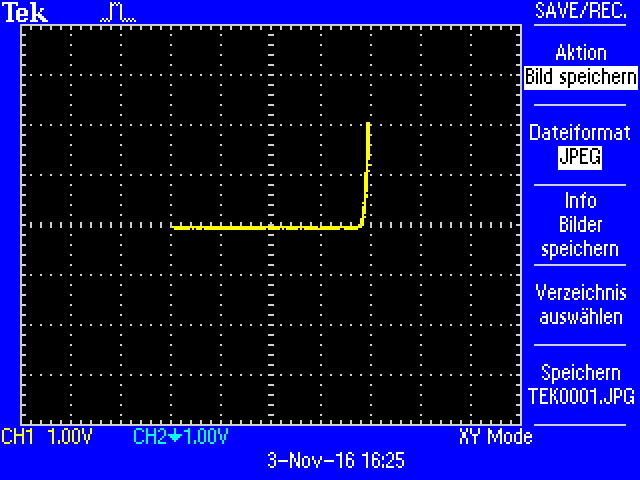
\includegraphics[scale=1]{Daten/TEK0001.JPG}
           \captionof{figure}[DurchlassGerSil]{Kennlinie der roten LED} 
         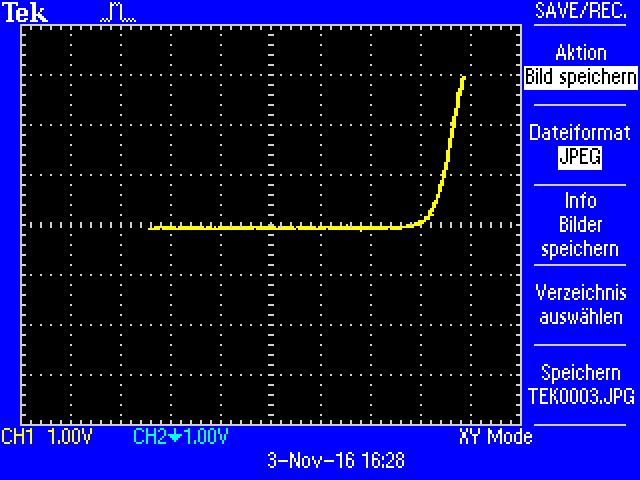
\includegraphics[scale=1]{Daten/TEK0003.JPG}
           \captionof{figure}[DurchlassGerSil]{Kennlinie der blauen LED} 
           \end{center}
        
       Die Schwellspannungen sind aus den Diagrammen abzulesen und sind:
       \begin{center}
       \begin{tabular}{c|c}
       &Schwellspannung\\ \hline
       Rot & $1,8 V$ \\
       Blau & $2,7 V$
       \end{tabular}
       \end{center}
       Damit lässt sich die Wellenlänge des Lichtes berechnen, das von der LED abgestrahlt wird.
       \begin{align*}
       		\lambda_{rot} & = \frac{h \cdot c}{e \cdot U_{rot}} \\
            & = \frac{6,626 \cdot 10^{-34} Js \cdot 0,3 \cdot 10^9 \frac{m}{s}}{1,6 \cdot 10^{-19} C \cdot 1,8 V} = 690,2 nm
       \end{align*} 
       \begin{align*}
       		\lambda_{blau} & = \frac{h \cdot c}{e \cdot U_{blau}} \\
            & = \frac{6,626 \cdot 10^{-34} Js \cdot 0,3 \cdot 10^9 \frac{m}{s}}{1,6 \cdot 10^{-19} C \cdot 2,7 V} = 460,1 nm
       \end{align*}
       
       Die errechneten Wellenlängen passen sehr gut zum Licht, dass von den LEDs abgestrahlt wird, wenn man für blaues Licht eine Wellenlänge von $420nm$ bis $490nm$ und $650nm$ bis $750nm$ für rotes Licht annimmt. \footnote{https://de.wikipedia.org/wiki/Licht}
	\pagebreak

    \chapter{Fehlerrechnung}
	Um das Ventilvolumen in die Formel einzubringen, wird $\gamma$ in Abhängigkeit der Länge $l$, statt der Fläche $A$ und dem Volumen $V$ geschrieben.
      \begin{align*}
     		\gamma = \frac{16 \pi \cdot m \cdot l \cdot f_0^2}{d^2 \cdot p_0}
      \end{align*}
      \begin{align*}
     		\Delta\gamma_{\text{Luft}} &= 
            \left| \frac{16\pi l f_0^2}{d^2 p_0}\right| \Delta m + 
            \left| \frac{16\pi m f_0^2}{d^2 p_0}\right| \Delta l + 
            \left| \frac{32\pi m l f_0}{d^2 p_0}\right| \Delta f_0 + 
            \left| -\frac{32 \pi m l f_0^2}{d^3 p_0}\right| \Delta d \\&+ 
            \left| -\frac{16 \pi m l f_0^2}{d^2 p_0^2}\right| \Delta p_0 \\&=
            \left| \frac{16\pi (0,45m + 0,001m) (13,4Hz)^2}{(0,016m)^2 (103100Pa)}\right| (0,0000001kg)\\ &+ 
            \left| \frac{16\pi (0,0088781kg) (13,4Hz)^2}{(0,016m)^2 (103100Pa)}\right| (0,001m) \\ &+ 
            \left| \frac{32\pi (0,0088781kg) (0,45m + 0,001m) (13,4Hz)}{(0,016m)^2 (103100Pa)}\right| (0,2Hz) \\ &+ 
            \left| -\frac{32 \pi (0,0088781kg) (0,45m + 0,001m) (13,4Hz)^2}{(0,016m)^3 (103100Pa)}\right| (0,00001m)\\&+ 
            \left| -\frac{16 \pi (0,0088781kg) (0,45m + 0,001m) (13,4Hz)^2}{(0,016m)^2 (103100Pa)^2}\right| (100Pa) \\ &= 0,048
      \end{align*} \\
      
      Analog für die weiteren Fehler
      \begin{center}
      \begin{tabular}{c|c}
$l ~[\text{m}]$ & $\Delta\gamma ~[1]$    \\ \hline
0,45         & 0,048 \\
0,40          & 0,045\\
0,35         & 0,045 \\
0,30          & 0,042 \\
0,25         & 0,039 \\
0,20          & 0,037 \\
0,15         & 0,036 \\
0,10          & 0,035	
		\end{tabular}
	\end{center}
      
\captionof{table}[]{Fehler für die Messung mit Luft als Kolbenfüllung.}
\begin{center}
      \begin{tabular}{c|c}
$l ~[\text{m}]$ & $\Delta\gamma ~[1]$    \\ \hline
0,45 & 0,048 \\
0,40  & 0,045 \\
0,35 & 0,042 \\
0,30  & 0,040 \\
0,25 & 0,038 \\
0,20  & 0,036 \\
0,15 & 0,035 \\
0,10  & 0,034
		\end{tabular}
	\end{center}
      
\captionof{table}[]{Fehler für die Messung mit Kohlenstoffdioxid als Kolbenfüllung.}

\begin{center}
      \begin{tabular}{c|c}
$l ~ [\text{m}]$ & $\Delta\gamma ~[1]$    \\ \hline
0,45   & 0,053 \\
0,40    & 0,050 \\
0,35   & 0,048 \\
0,30    & 0,045 \\
0,24   & 0,042 \\
0,19   & 0,038 \\
0,14   & 0,047 \\
0,095  & 0,038 
		\end{tabular}
	\end{center}
      
\captionof{table}[]{Fehler für die Messung mit Argon als Kolbenfüllung.}
\ \\
Es soll nur ein Wert für den Fehler angegeben werden. Anstatt wie bei den Messwerten zu mitteln, wird hier jedoch der größte Fehler angenommen, damit der Fehlerwert nicht zu gering ausfällt.

\begin{align*}
 	\Delta \gamma_{\text{Luft}} & = 0,048\\
    \Delta \gamma_{\text{CO}_2} & = 0,048\\
    \Delta \gamma_{\text{Argon}}& = 0,053
\end{align*}

     	\section{Mögliche Abweichungen}
        	Im Versuch wird angenommen, dass die Erregerfrequenz beim Maximum der Schwingung der Eigenfrequenz des ungedämpften Systems entspricht. Durch Dämpfung fällt die Frequenz jedoch geringer aus, was sich durch den Zusammenhang $\gamma \propto f^2$ stark auf das Ergebnis auswirkt. Der Wert für den gemessenen Adiabatenexponent liegt also unter dem tatsächlichen. Außerdem wird nicht mit einem isolierten System gemessen, sodass der Vorgang nicht vollständig adiabatisch verläuft. Reibung verursacht ebenfalls einen Fehler.
	\pagebreak
    
	\chapter{Zusammenfassung}
In diesem Versuch konnte die Arrhenius-Andrade-Beziehung der expotentiellen Temperaturabhänigkeit der Viskosität bestätigt werden. \\
\\
Als Wert der stoffabhängigen Konstanten erhielt man einen Wert von
\begin{center}
\begin{tabular}{c|c}
Konstante & Wert \\ \hline
$c_1$ & $(3,5 \cdot 10^{-9} \pm 0,33 \cdot 10^{-9}) Pa \cdot s $ \\
$c_2$ &  $(5249,64 \pm 131,17) K $\\
\end{tabular}
\end{center}

Die Viskositäten in Abhängigkeit der Temperatur:
\begin{center}
   \begin{tabular}{c|c|c}
  		Temperatur $T [\si{\kelvin}]$ & Fallzeit $t [\si{\second}]$ & Viskosität $\eta [\si{\pascal\second}]$ \\ \hline \hline
        298,25 & 38,784	& 0,1538 \\
		308,25 & 20,994	& 0,0832 \\
		318,25 & 13,138	& 0,0521 \\
		328,25 & 7,806	& 0,0310 \\
		333,25 & 6,336	& 0,0251 \\
   \end{tabular}
   \captionof{table}[]{Werte der dynamischen Viskosität}
   \end{center}
   Dabei ist der Fehler jeweils $\Delta \eta = 0,002 Pas$
   

\pagebreak
	\chapter{Anhang}
    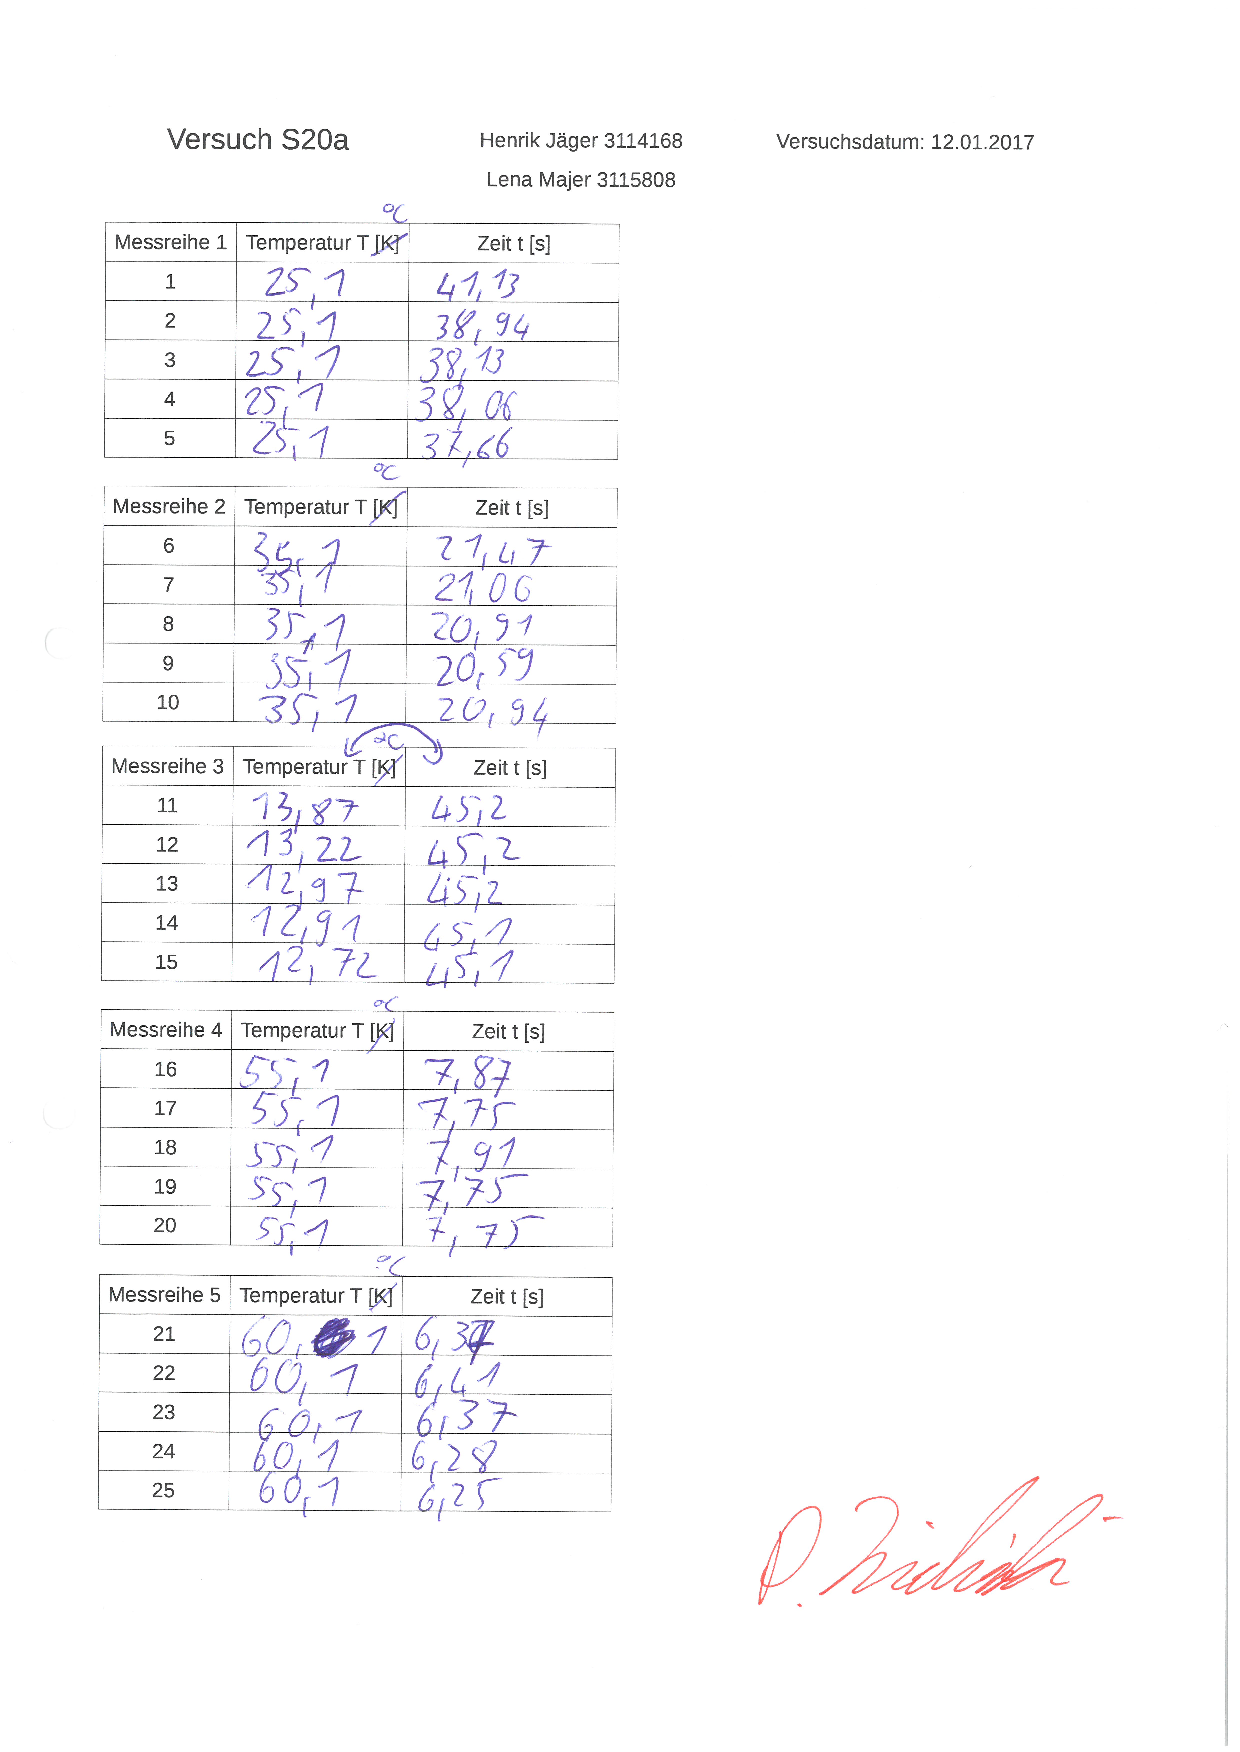
\includegraphics[scale=0.6]{protokoll.pdf}
    \captionof{figure}[]{Messprotokoll}
	










\end{document}
